% !TEX root = ../../../main.tex
\begin{figure}
    \centering
    \subfigure[自变量的参数估计]{
    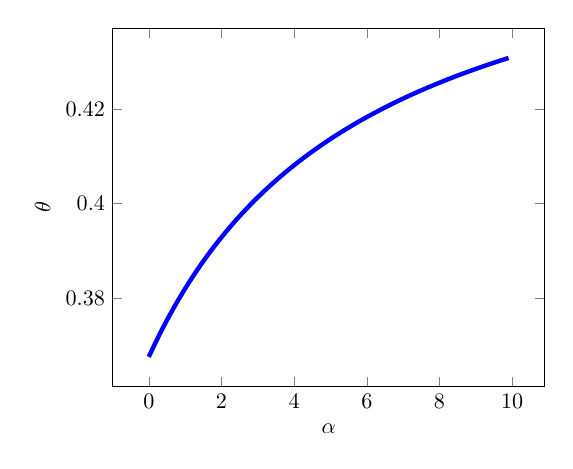
\begin{tikzpicture}[scale=0.8]
        \begin{axis}[xlabel={$\alpha$}, ylabel={$\theta$},clip marker paths=true]
            \addplot+[no marks,line width=2pt] coordinates{
(0.0, 0.3676867322464298)
(0.1, 0.3693365400220552)
(0.2, 0.3709337670622458)
(0.3, 0.37248088428726317)
(0.4, 0.3739802101843202)
(0.5, 0.3754339223836698)
(0.6, 0.37684406819557087)
(0.7, 0.37821257421530985)
(0.8, 0.3795412550910811)
(0.9, 0.38083182153854145)
(1.0, 0.3820858876766342)
(1.1, 0.38330497775066596)
(1.2, 0.3844905323015613)
(1.3, 0.3856439138339568)
(1.4, 0.386766412029656)
(1.5, 0.38785924854884746)
(1.6, 0.38892358145626177)
(1.7, 0.3899605093062256)
(1.8, 0.39097107491682526)
(1.9, 0.3919562688603964)
(2.0, 0.39291703269501477)
(2.1, 0.39385426195898954)
(2.2, 0.3947688089485273)
(2.3, 0.39566148529661116)
(2.4, 0.39653306436945324)
(2.5, 0.39738428349549926)
(2.6, 0.3982158460403468)
(2.7, 0.399028423340026)
(2.8, 0.39982265650364646)
(2.9, 0.40059915809565255)
(3.0, 0.40135851370701625)
(3.1, 0.4021012834237232)
(3.2, 0.40282800320038914)
(3.3, 0.40353918614604983)
(3.4, 0.40423532372855975)
(3.5, 0.4049168869036779)
(3.6, 0.4055843271741023)
(3.7, 0.4062380775836048)
(3.8, 0.4068785536508389)
(3.9, 0.40750615424698455)
(4.0, 0.4081212624211984)
(4.1, 0.4087242461774313)
(4.2, 0.40931545920589063)
(4.3, 0.40989524157231194)
(4.4, 0.4104639203676965)
(4.5, 0.41102181032126595)
(4.6, 0.41156921437899907)
(4.7, 0.41210642424994615)
(4.8, 0.4126337209224423)
(4.9, 0.41315137515214406)
(5.0, 0.41365964792362075)
(5.1, 0.4141587908871698)
(5.2, 0.4146490467724555)
(5.3, 0.4151306497802951)
(5.4, 0.41560382595401424)
(5.5, 0.4160687935315291)
(5.6, 0.4165257632793851)
(5.7, 0.4169749388097651)
(5.8, 0.41741651688151116)
(5.9, 0.4178506876860248)
(6.0, 0.418277635119078)
(6.1, 0.4186975370390905)
(6.2, 0.41911056551292514)
(6.3, 0.41951688704972484)
(6.4, 0.41991666282345586)
(6.5, 0.42031004888494505)
(6.6, 0.42069719636380987)
(6.7, 0.4210782516609269)
(6.8, 0.42145335663197425)
(6.9, 0.4218226487624249)
(7.0, 0.42218626133458476)
(7.1, 0.42254432358697236)
(7.2, 0.42289696086654793)
(7.3, 0.42324429477407977)
(7.4, 0.4235864433030563)
(7.5, 0.42392352097248265)
(7.6, 0.4242556389538037)
(7.7, 0.42458290519236197)
(7.8, 0.4249054245235662)
(7.9, 0.4252232987840827)
(8.0, 0.4255366269183148)
(8.1, 0.4258455050803364)
(8.2, 0.42615002673156777)
(8.3, 0.42645028273439956)
(8.4, 0.42674636144188083)
(8.5, 0.42703834878377267)
(8.6, 0.42732632834905204)
(8.7, 0.4276103814650764)
(8.8, 0.42789058727357754)
(8.9, 0.42816702280356334)
(9.0, 0.42843976304138476)
(9.1, 0.42870888099796833)
(9.2, 0.42897444777345606)
(9.3, 0.4292365326193113)
(9.4, 0.42949520299800126)
(9.5, 0.42975052464041735)
(9.6, 0.43000256160104855)
(9.7, 0.430251376311115)
(9.8, 0.4304970296296483)
(9.9, 0.4307395808926763) 

		};

		\end{axis}
	\end{tikzpicture}
            }
            \subfigure[偏置项的参数估计]{
    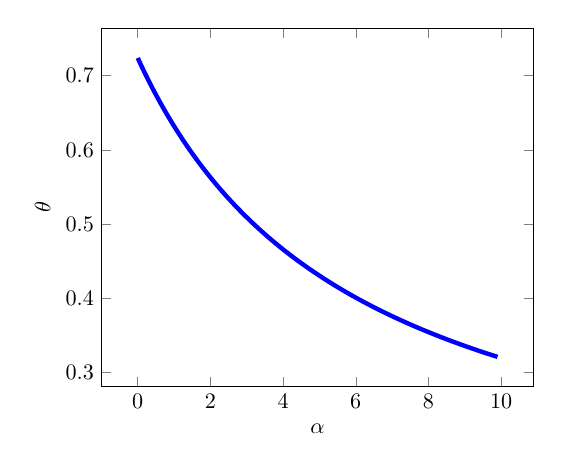
\begin{tikzpicture}[scale=0.8]
        \begin{axis}[xlabel={$\alpha$}, ylabel={$\theta$},clip marker paths=true]
            \addplot+[no marks,line width=2pt] coordinates{
            (0.0, 0.7237361931657513)
(0.1, 0.7132268005733423)
(0.2, 0.7030518803866128)
(0.3, 0.6931957147900694)
(0.4, 0.6836435556130112)
(0.5, 0.6743815506923666)
(0.6, 0.6653966768460097)
(0.7, 0.6566766787739579)
(0.8, 0.6482100132849223)
(0.9, 0.6399857983146978)
(1.0, 0.6319937662621747)
(1.1, 0.6242242212231529)
(1.2, 0.6166679997467152)
(1.3, 0.6093164347801888)
(1.4, 0.6021613225053459)
(1.5, 0.5951948917975493)
(1.6, 0.5884097760704604)
(1.7, 0.5817989872903184)
(1.8, 0.5753558919681846)
(1.9, 0.5690741889565565)
(2.0, 0.5629478888933831)
(2.1, 0.5569712951538563)
(2.2, 0.5511389861811812)
(2.3, 0.545445799082179)
(2.4, 0.5398868143830478)
(2.5, 0.5344573418506202)
(2.6, 0.5291529072932707)
(2.7, 0.5239692402633291)
(2.8, 0.5189022625900337)
(2.9, 0.5139480776786917)
(3.0, 0.5091029605160546)
(3.1, 0.5043633483289844)
(3.2, 0.4997258318470159)
(3.3, 0.49518714712295614)
(3.4, 0.49074416787180714)
(3.5, 0.4863938982883892)
(3.6, 0.4821334663108038)
(3.7, 0.47796011729647914)
(3.8, 0.4738712080822002)
(3.9, 0.46986420140134405)
(4.0, 0.46593666063302197)
(4.1, 0.4620862448606689)
(4.2, 0.45831070421912545)
(4.3, 0.45460787551012954)
(4.4, 0.45097567806924027)
(4.5, 0.4474121098666556)
(4.6, 0.44391524382733366)
(4.7, 0.4404832243555672)
(4.8, 0.4371142640513467)
(4.9, 0.43380664060601615)
(5.0, 0.43055869386596407)
(5.1, 0.4273688230538884)
(5.2, 0.4242354841377907)
(5.3, 0.4211571873385977)
(5.4, 0.41813249476809383)
(5.5, 0.4151600181890818)
(5.6, 0.4122384168907106)
(5.7, 0.4093663956718579)
(5.8, 0.406542702926319)
(5.9, 0.4037661288241032)
(6.0, 0.4010355035825672)
(6.1, 0.39834969582323926)
(6.2, 0.3957076110085268)
(6.3, 0.3931081899541582)
(6.4, 0.3905504074134702)
(6.5, 0.38803327072871546)
(6.6, 0.3855558185466057)
(6.7, 0.38311711959386585)
(6.8, 0.3807162715097868)
(6.9, 0.378352399733059)
(7.0, 0.3760246564391938)
(7.1, 0.3737322195267116)
(7.2, 0.37147429164880474)
(7.3, 0.3692500992886607)
(7.4, 0.36705889187575175)
(7.5, 0.3648999409411756)
(7.6, 0.3627725393102501)
(7.7, 0.36067600032990993)
(7.8, 0.35860965712973963)
(7.9, 0.3565728619147048)
(8.0, 0.3545649852877406)
(8.1, 0.35258541560146894)
(8.2, 0.3506335583367591)
(8.3, 0.348708835507196)
(8.4, 0.34681068508863594)
(8.5, 0.3449385604717268)
(8.6, 0.34309192993708415)
(8.7, 0.34127027615181305)
(8.8, 0.33947309568601053)
(8.9, 0.33769989854906546)
(9.0, 0.33595020774395035)
(9.1, 0.3342235588395504)
(9.2, 0.33251949955945587)
(9.3, 0.3308375893869478)
(9.4, 0.32917739918527916)
(9.5, 0.32753851083254604)
(9.6, 0.3259205168705261)
(9.7, 0.3243230201668966)
(9.8, 0.3227456335901433)
(9.9, 0.32118797969680885)
          
        };


        \end{axis}
    \end{tikzpicture}
            
            }
\caption{岭迹线\label{fig:L2_ridge_trace}}
\end{figure}
